\lab{Pseudospectra}{Pseudospectra}
\label{lab:pseudospectra}
\objective{The Pseudospectrum of a matrix is related to its eigenvalues.  The Pesudospectra of normal and non-normal matrices will be investigated.  We will plot pseudospectra and examine the characteristics of different types of matrices.}



\section*{Pseudospectra Definition}
Eigenvalues of matrices are extremely important, as there are a myriad of practical applications in which they are used.  In Quantum Mechanical systems, particularly, many operators can be represented by matrices, and the eigenvalues are the physical observables of the system.  Though we can make extremely precise measurements, there is often an $\epsilon$-small error in measurements.  In this case, we are interested not just in the eigenvalues, but in the ``almost" eigenvalues, the $\epsilon$ region surrounding the actual eigenvalue.  The $\epsilon$ region around the eigenvalues of a square matrix $A$ represents the $\epsilon$-pseudospectrum (plural \emph{pseudospectra}) of $A$, which can be denoted $\sigma_{\epsilon}(A)$.

To be more precise, the \emph{point spectrum} of $A$ is defined as
\begin{align*}
	\sigma(A)&=\{z \in \mathbb{C}: det(zI-A)=0\}\\
	&=\{z \in \mathbb{C}: (zI-A)^{-1} \text{ is undefined}\}.
\end{align*}
The point spectrum of $A$ contains all the eigenvalues of $A$.  By convention, if $z$ is an eigenvalue of $A$, then $\|(zI-A)^{-1}\|=\infty$.
The $\epsilon$-pseudospectrum of a matrix is a generalization of its point spectrum, and for a matrix $A$ is defined as
\begin{equation}
	\sigma_{\epsilon}(A)=\{z \in \mathbb{C}:\|(zI-A)^{-1}\| > \epsilon^{-1}\}.
\end{equation}
Note that this definition requires the use of a matrix norm. Any matrix norm can be used, but in this lab we will use the norm induced by the 2-norm.

In the case of the 2-norm, the pseudospectrum has an equivalent definition:
\begin{equation}
	\label{equ:spec}
	\sigma_{\epsilon}(A)=\{z \in \mathbb{C}: z \in \sigma(A+E) \text{ for some $E$ with } \|E\|<\epsilon\}.
\end{equation}
When the entries of a matrix are slightly altered, changes in the point spectrum also occur.  The pseudospectrum can then be thought of as the set of eigenvalues that can result from small changes in the entries of a matrix.  If $A$ is an $n \times n$ matrix, then we can use Equation \ref{equ:spec} with some $n \times n$ matrix $E$ satisfying $\lVert E \rVert < \epsilon$ to find the $\epsilon$-pseudospectrum of $A$, which will be a set of all complex numbers $z$ which are in the point spectrum of $A+E$.

One means of plotting the $\epsilon$-pseudospectrum of $A$ is by generating several random matrices $E$ with norm $\epsilon$, and then plotting the eigenvalues $z$ of all of them together.  The horizontal axis is the real part of $z$, with the vertical axis being the imaginary part of $z$.

\begin{figure}
\begin{center}
\begin{subfigure}[b]{.49\textwidth}
\centering
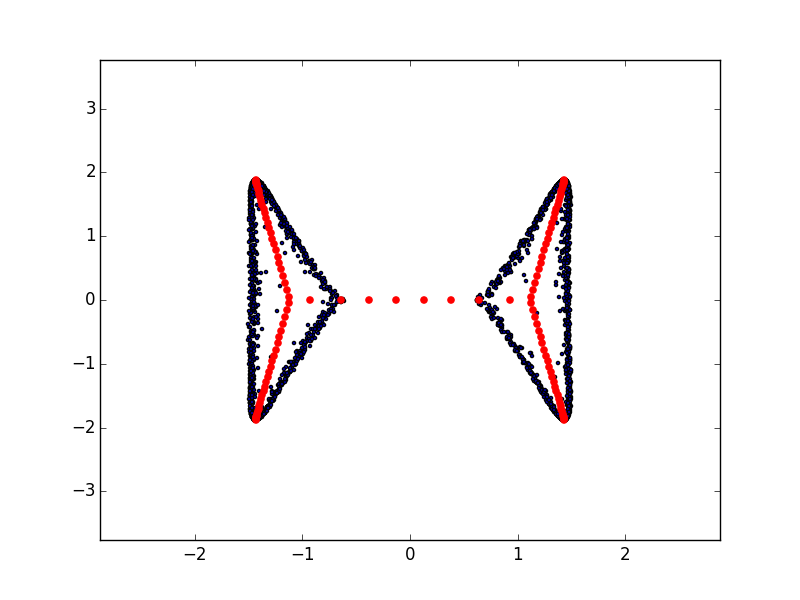
\includegraphics[width=\textwidth]{ps_scatter1}
\end{subfigure}
\begin{subfigure}[b]{.49\textwidth}
\centering
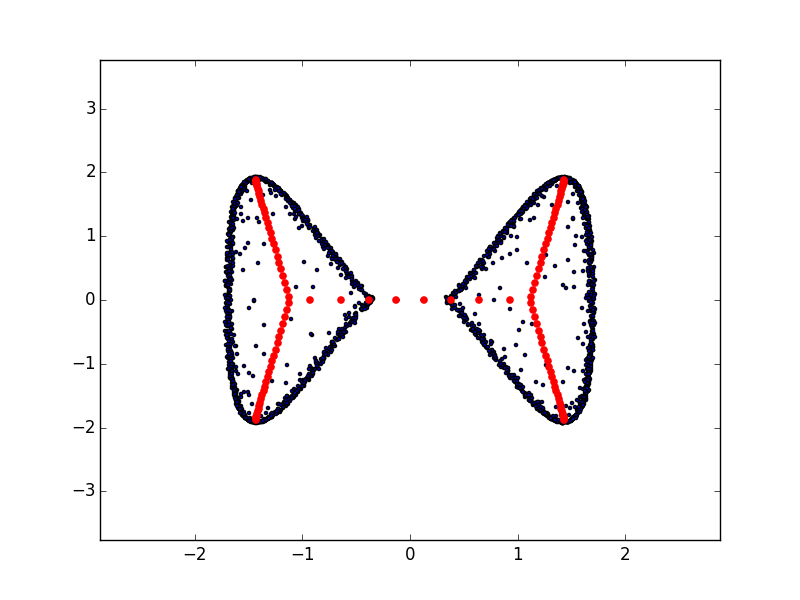
\includegraphics[width=\textwidth]{ps_scatter2}
\end{subfigure}
\caption{Scatter plots representing the $\epsilon$-pseudospectrum of the matrix given in Problem 1. The plot on the left uses $\epsilon=10^{-6}$. The plot on the right uses $\epsilon=10^{-3}$. In both plots, the eigenvalues of twenty matrices $A+E$ were plotted.}
\label{fig:ps_scatter}
\end{center}
\end{figure}

\begin{problem}
Complete the function below for plotting the pseudospectrum of a matrix $A$ by plotting the point spectra of several matrices $A+E$, where $\lVert E \rVert = \epsilon$. 

\begin{lstlisting}
def ps_scatter_plot(A, epsilon=.001, num_pts=20):
    '''Plots the 'poorman's pseudospectrum' of a matrix A
    
    Parameters:
    A : ndarray of size (n,n)
        The matrix whose pseudospectrum is to be plotted.
    epsilon : float
        The norm of the random matrices that are generated.
        Defaults to 10**-3
    num_pts : int
        The number of matrices, E, that will be used in the
        algorithm. Defaults to 20.       
    '''
\end{lstlisting}

To get random matrices of the right norm, generate random matrices, divide them by their respective 2-norms, and then multiply by epsilon.
Have your code plot the eigenvalues (point spectrum) of $A$ in one color, and the point spectrum of each $A+E$ in a different color.  The $\epsilon$-pseudospectrum of $A$ can be though of as the region enclosed by your points.  Test your code on the 120x120 matrix:
\begin{equation}
	\begin{pmatrix}
		0  &  i  &  -1  &  0  & \cdots  &  0  \\
		-i &  0  &   i  & -1 & \ddots  &  \vdots  \\
		1  & -i  &   0  &  i &\ddots&  0  \\
		0   & 1 & -i & 0 &\ddots& -1\\
		\vdots   & \ddots    & \ddots & \ddots &\ddots & i\\
		 0  &  \cdots     &   0     &    1  &   -i  & 0
		\end{pmatrix}
\label{prob:pseudoplot}
\end{equation}

Your plot should resemble those in Figure \ref{fig:ps_scatter}.
\end{problem}

This method of plotting, often called the ``poorman's pseudospectrum", can only show the $\epsilon$-pseudospectrum of $A$ for one value of $\epsilon$ at a time, and even then it just provides a bound for the pseudospectrum. In many cases it does not give sufficient information, so we will now explain how to plot the $\epsilon$-pseudospectrum using a more precise algorithm.

\section*{An Equivalent Pseudospectral Definition}

Recall the following definition:

\begin{equation}
\sigma _{\epsilon}(A) = \{ z \in \mathbb{C} \, : \, \lVert (zI_n-A)^{-1} \rVert > \epsilon ^{-1}\}	.
\end{equation}

When we are using the induced 2-norm, we get that $\lVert (zI_n-A)^{-1} \rVert$ is the largest singular value of $(zI_n-A)^{-1}$.  This is also defined for a matrix $B$ as the square root of the largest eigenvalue of $B^{H} B$ 
 This is equal to $1/s_{min}(zI_n-A)$, where $s_{min}(zI_n-A)$ is the smallest singular of $(zI_n-A)$. Hence, we can write

\begin{equation}
\sigma _{\epsilon}(A) = \{ z \in \mathbb{C} \, | \, s_{min}(A-zI_n) < \epsilon \}.	
\end{equation}


\section*{The Lanczos Method}

Using this new definition for $\sigma _{\epsilon}(A)$, we can now plot pseudospectra using Lanczos iterations. Lanczos iterations make use of the Arnoldi method described in Lab \ref{lab:kry_arnoldi} in order to more efficiently compute the smallest eigenvalue of $(zI_n-A)$. This method allows us to plot the pseudospectrum as a contour plot, where each contour corresponds to a fixed value of $\epsilon$. The algorithm is provided below.

\begin{algorithm}
\begin{algorithmic}[1]
\Procedure{Pseudospectrum}{$A, m, epsilon$}
	\State $T \gets schur(A)$			\Comment{Compute the Schur decomposition of A}
	\State $eigsA \gets diagonal(T)$
	\State $xvals,yvals \gets psgrid(eigsA,m)$
	\State $sigmin \gets \zeros{m}{m}$					
	\For{$k=0\ldots m-1$}
	    \For{$j=0\ldots m-1$}		
		    \State $T_1 \gets (xvals[k]+i*yvals[j])I_n-T$  
		    \State \Comment{$I_n$ is the $n\times n$ identity matrix.}
		    \State $T_2 \gets T1^*$        \Comment{Compute the conjugate transpose.}		
		    \State $sigold \gets 0$    \Comment{Initialize variables.}
		    \State $qold \gets \zeros{n}{1}$
		    \State $beta \gets 0$
		    \State $H \gets \zeros{n}{n}$
		    \State $q \gets$ random, complex-valued $n \times 1$ array of norm 1 
		    \State \Comment{Assume both real and imaginary parts are normally distributed}
		    \For{$p=0 \ldots N-2$}
			    \State $b_1 \gets$ solution to $T_2x = q$	
			    \State $b_2 \gets$ solution to $T_1x = b_1$
			    \State $v \gets b_2 - beta*qold$
			    \State $alpha \gets real(q^**v)$
			    \State $v \gets v - alpha*q$
			    \State $beta \gets \norm{v}$
			    \State $qold \gets q$
			    \State $q \gets v/beta$
			    \State $H[p+1,p] \gets beta$
			    \State $H[p,p+1] \gets beta$
			    \State $H[p,p] \gets alpha$
			    %\State $eigsH \gets$ eigenvalues of $H[:p+1,:p+1]$
			    \State $sig \gets$ absolute value of largest eigenvalue of $H[:p+1,:p+1]$
			    \If{$|sigold/sig-1|<0.001$}
			        \State Break    \Comment{End loop if $sig$ is close to $sigold$}
			    \EndIf
			    \State $sigold \gets sig$
			\EndFor
			\State $sigmin[j,k] \gets \sqrt{sig}$
	    \EndFor
	\EndFor
	\State Plot the log of the values in $sigmin$ as a contour plot on the grid determined by $xvals$ and $yvals$.
\EndProcedure
\end{algorithmic}
\caption{The Lanczos Method. This algorithm accepts a $n \times n$ square matrix, $A$; a list of values for $\epsilon$; and an accuracy measure of $m$. It computes the $10^{-\epsilon}$-pseudospectrum of $A$ for each value of $\epsilon$ and produces the contour plot on the grid determined by $xvals$ and $yvals$ as returned by psgrid().}
\label{alg:lanczos_method}
\end{algorithm}

Note that while this algorithm gives better results than our previous method of plotting pseudospectra, it is much slower.

\begin{figure}
\begin{center}
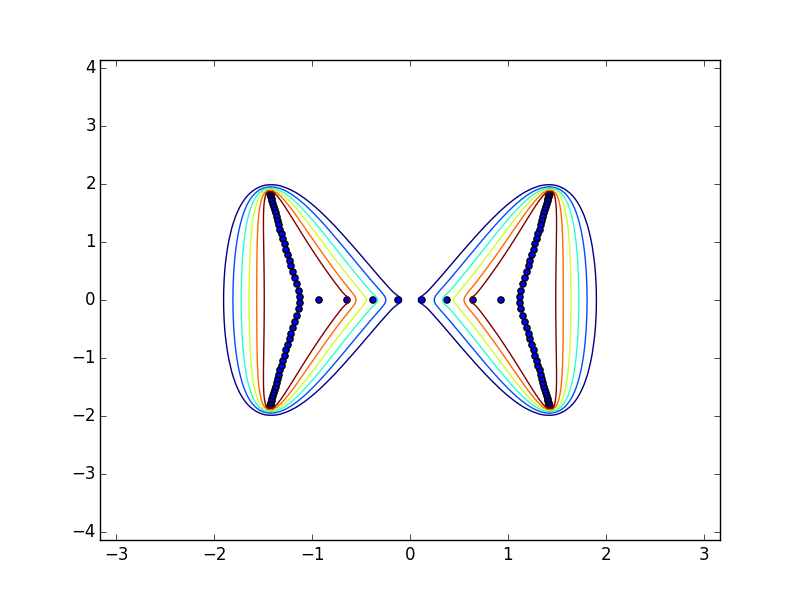
\includegraphics[width=\textwidth]{ps_contour}
\caption{Contour plot of the $\epsilon$-pseudospectrum of the matrix given in Problem 1, with $\epsilon=10^{-2},10^{-3},\cdots,10^{-7}$. }
\label{fig:ps_contour}
\end{center}
\end{figure}



\begin{problem}
Finish the function below for implementing Algorithm \ref{alg:lanczos_method} in Python. Make the function also plot the eigenvalues of the matrix on the same plot.

\begin{lstlisting}
def ps_contour_plot(A, m = 20, epsilon_vals=None):
    '''Plots the pseudospectrum of the matrix A as a contour plot.  Also,
    plots the eigenvalues.
    
    Parameters:
        A : square, 2D ndarray
            The matrix whose pseudospectrum is to be plotted
        m : int
            accuracy
        epsilon_vals : list of floats
            If k is in epsilon_vals, then the epsilon-pseudospectrum
            is plotted for epsilon=10**-k
            If epsilon_vals=None, the defaults of plt.contour() are used
            instead of any specified values.
     '''
    
\end{lstlisting}

Test your code on the matrix from Problem 1. Your plot should look like Figure \ref{fig:ps_contour}. You will need to choose a grid on which to plot the values computed in this algorithm. Use a grid that is roughly twice as large as one needed to plot the eigenvalues. To make your code run faster, make sure to use functions designed for Hermitian or triangular matrices whenever possible.
\begin{enumerate}
\item Plot the eigenvalues and contour lines on a complex plane.
\item $m$ defaults to 20 but if you want the plot to look like Figure \ref{fig:ps_contour}, you will need m to be close to 150.  Note that this will take a while longer.
\item In order to plot the contour lines.  Use the following code.
\begin{lstlisting}
plt.contour(xvals,yvals,np.log10(sigmin), levels=epsilon_vals)
\end{lstlisting}
\end{enumerate}

\end{problem}

\section*{Hermitian, Normal, and Nonnormal Matrices}
Recall that a matrix $A$ is Hermitian if it is equal to its conjuage transpose, i.e. $A^{H} = A$.  All the eigenvalues of Hermitian matrices are real.  However, if the elements change slightly (adding $E$), these matrices quickly fall out of the class of Hermitian matrices, and the $\epsilon$-pseudospectra may gain an imaginary component.

A broader class of matrices that includes all Hermitian matrices is the class of \emph{normal matrices}.  A normal matrix commutes with its conjugate transpose, i.e. $A A^{H} = A^{H} A$. In the case that $A$ is normal, it can be shown that the $\epsilon$-pseudospectrum consists of the union of circular sets about each of the eigenvalues of $A$. When $A$ is not a normal matrix, the pseudospectrum can have more varied shapes. Because of this, plotting the pseudospectrum of a nonnormal matrix can provide more information about its behavior.

Figure \ref{fig:ps_normal} provides an example of this. The plots show the pseudospectra of the matrices:

\begin{equation}
	B = \begin{pmatrix}
		-1 & 0 & 0\\
		0 & 1 & 0\\
		0 & 0 & i
	\end{pmatrix}, \qquad 	B' = \begin{pmatrix}
		-1 & -1 & -1\\
		0 & 1 & 1\\
		0 & 0 & i
	\end{pmatrix}.
\end{equation}

Note that these matrices have the same set of eigenvalues, but that while $B$ is normal, $B'$ is not. The plot of the pseudospectrum of $B$ shows the expected circular regions, but the plot for $B'$ lacks such symmetry. Another example of this can be seen in Figure \ref{fig:ps_scatter}. The pseudospectrum does not expand out from all of the eigenvalues evenly. Most of the region contained in the pseudospectrum lies on the sides of the plot, and not close to the center.\\

Because the pseudospectra of normal matrices behave so consistently, the study of pseudospectra focuses on nonnormal matrices. Pseudospectra can also be used to study infinite-dimensional linear operators, but different methods are required for plotting their pseudospectra.

\begin{figure}
\begin{center}
\begin{subfigure}[b]{.49\textwidth}
\centering
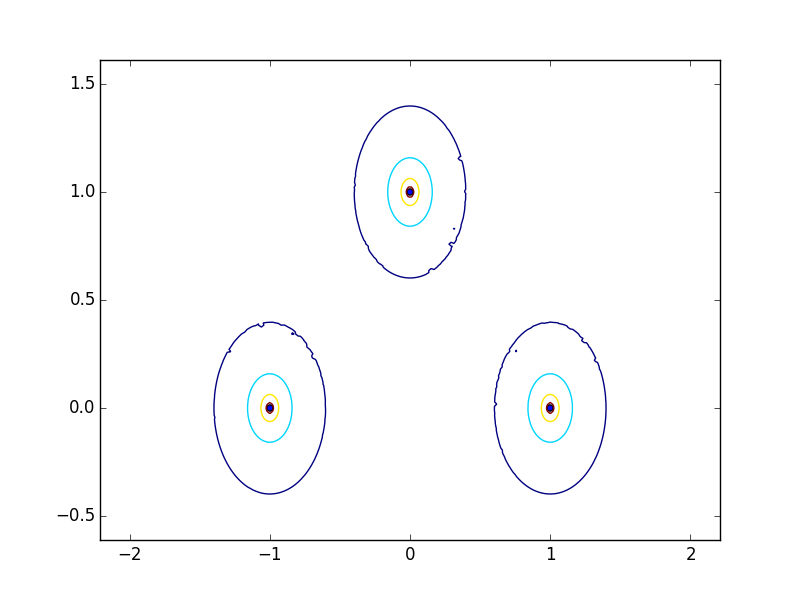
\includegraphics[width=\textwidth]{ps_normal}
\end{subfigure}
\begin{subfigure}[b]{.49\textwidth}
\centering
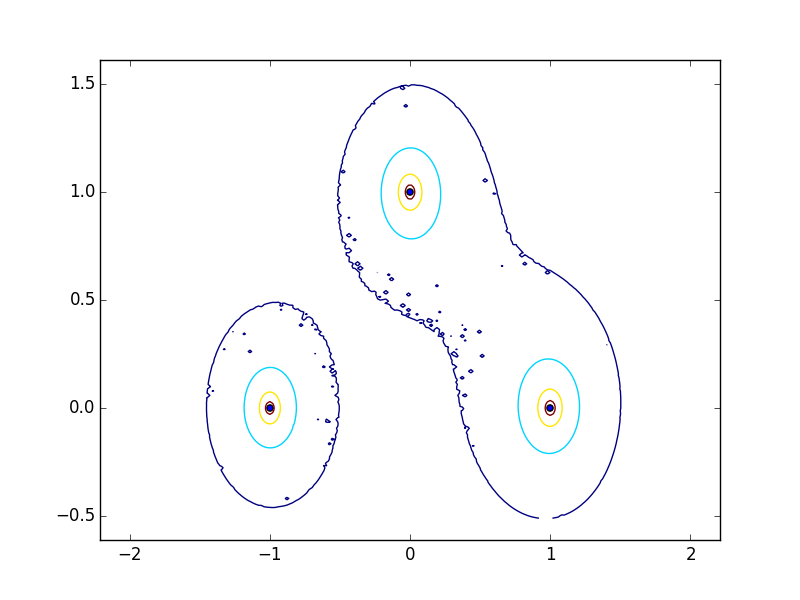
\includegraphics[width=\textwidth]{ps_nonnormal}
\end{subfigure}
\caption{Plots of the Pseudospectrum of two matrices with the same eigenvalues. The plot on the left is for a normal matrix, and the one on the right is for a nonnormal matrix. The contours correspond to $\epsilon=10^{-0.4},10^{-0.8},10^{-1.2}$}
\label{fig:ps_normal}
\end{center}
\end{figure}

\begin{problem}
Using your function from problem \ref{prob:pseudoplot}, investigate how the pseudospectra of Nonnormal, Hermitian, and Normal matrices differ.  To do so, use the matrix given in problem \ref{prob:pseudoplot} as the Nonnormal matrix.  

For the Hermitian matrix, change the subdiagonal of $1$s to be $-1$.  

For the Normal matrix, reset all of the subdiagonal entries to be zero (change the $1$ diagonal and $-i$ diagonal to zeros).  Set all of the diagonal entries to be random complex values (so as to get different eigenvalues).

Plot your results.
\end{problem} 


% ~\cite{Tufte2005}
